 \documentclass[12pt]{article}
\usepackage[utf8]{inputenc}
\usepackage[spanish,es-lcroman, es-tabla]{babel}
\usepackage[autostyle,spanish=mexican]{csquotes}
\usepackage{amsmath}
\usepackage{amssymb}
\usepackage{nccmath}
\numberwithin{equation}{section}
\usepackage{amsthm}
\usepackage{graphicx}
\usepackage{epstopdf}
\DeclareGraphicsExtensions{.pdf,.png,.jpg,.eps}
\usepackage{color}
\usepackage{float}
\usepackage{multicol}
\usepackage{enumerate}
\usepackage[shortlabels]{enumitem}
\usepackage{anyfontsize}
\usepackage{anysize}
\usepackage{array}
\usepackage{multirow}
\usepackage{enumitem}
\usepackage{cancel}
\usepackage{tikz}
\usepackage{circuitikz}
\usepackage{tikz-3dplot}
\usetikzlibrary{babel}
\usetikzlibrary{shapes}
\usepackage{bm}
\usepackage{mathtools}
\usepackage{esvect}
\usepackage{hyperref}
\usepackage{relsize}
\usepackage{siunitx}
\usepackage{physics}
%\usepackage{biblatex}
\usepackage{standalone}
\usepackage{mathrsfs}
\usepackage{bigints}
\usepackage{bookmark}
\spanishdecimal{.}

\setlist[enumerate]{itemsep=0mm}

\renewcommand{\baselinestretch}{1.5}

\let\oldbibliography\thebibliography

\renewcommand{\thebibliography}[1]{\oldbibliography{#1}

\setlength{\itemsep}{0pt}}
%\marginsize{1.5cm}{1.5cm}{2cm}{2cm}


\newtheorem{defi}{{\it Definición}}[section]
\newtheorem{teo}{{\it Teorema}}[section]
\newtheorem{ejemplo}{{\it Ejemplo}}[section]
\newtheorem{propiedad}{{\it Propiedad}}[section]
\newtheorem{lema}{{\it Lema}}[section]

%\author{M. en C. Gustavo Contreras Mayén. \texttt{curso.fisica.comp@gmail.com}}
\title{Sistemas Coordenados \\ {\large Matemáticas Avanzadas de la Física}\vspace{-1.5\baselineskip}}
\date{ }
\author{}
\begin{document}
%\renewcommand\theenumii{\arabic{theenumii.enumii}}
\renewcommand\labelenumii{\theenumi.{\arabic{enumii}}}
\maketitle
\fontsize{14}{14}\selectfont
\section{Introducción.}
Buena parte de la formación que hemos recibido tanto en la matemática como en la física, se ha hecho mediante un sistema de referencia cartesiano, donde ya conoces al conjunto de vectores cartesianos $\mathbf{i}$, $\mathbf{j}$, $\mathbf{k}$, que sabemos que son constantes en dirección y en magnitud. 
\par
En ciertos problemas se puede introducir una distancia radial $\mathbf{r}$, que se puede manejar incluso como una función de $x$, $y$, $z$. Desafortunadamente, no todos los problemas físicos se ajustan a una solución en coordenadas cartesianas. Por ejemplo, si tenemos un problema fuerza central, $\mathbf{F} = \va{r} \: F(r)$, como en el caso de la fuerza gravitacional o electrostática, el uso de coordenadas cartesianas resulta ser inadecuado. Tal problema exige el uso de un sistema de coordenadas en el que se toma la distancia radial como una de las coordenadas, es decir, usamos un sistema de coordenadas esféricas.
\par
El punto es que el sistema coordenado debe de seleccionarse de modo que se adapte al problema, para aprovechar cualquier oportunidad o simetría presente en el mismo. Luego, con buena disposición, resultará más fácil la solución que cuando se obliga a adaptar una estructura cartesiana. Cuando se menciona \enquote{de más fácil solución}, significa que se tendrá una ecuación diferencial parcial (EDP) que puede separarse en ecuaciones diferenciales ordinarias (EDO), frecuentemente en la \enquote{forma estándar} en el nuevo sistema coordenado. La \emph{técnica de separación de variables}, se verá en el Tema 2 del curso.
\par
Nos va a interesar aquellos sistemas de coordenadas en donde la ecuación
\begin{align}
\nabla^{2} \psi + k^{2} \: \psi = 0
%\label{eq:ecuacion_02_01}
\end{align}
es una ecuación separable.  En particular ésta ecuación tiene como particular el hecho de que si:
\begin{itemize}
\item $k^{2} = 0$, se obtiene la ecuación de Laplace.
\item $k^{2} = (+) \mbox{ constante}$, se obtiene la ecuación de Helmholtz.
\item $k^{2} = (-) \mbox{ constante}$, se obtiene la ecuación de difusión (en su parte espacial).
\item $k^{2} = \mbox{ constante } \times \mbox{ energía cinética}$, se obtiene la ecuación de onda de Schrödinger.
\end{itemize}
Se ha demostrado que existen once sistemas coordenados en donde la ec. de Helmholtz puede separarse. 
\par
Naturalmente, hay un costo que se debe pagar por el uso de un sistema diferente al de coordenadas cartesianas. Todavía no hemos escrito las expresiones para el gradiente, la divergencia, o el rotacional en los sistemas de coordenadas no cartesianas. Primero debemos desarrollar un sistema de coordenadas curvilíneas, un sistema general que pueda especializarse para cualquiera de los sistemas coordenados particulares de interés. Comenzaremos con esta parte en el primer tema del curso. 
\subsection{Coordenadas curvilíneas.}
En coordenadas cartesianas nos ocupamos de tres familias de planos mutuamente perpendiculares: $x = \mbox{ constante}$, $y = \mbox{ constante}$, y $z = \mbox{ constante}$. Imaginemos que superponemos en este sistema otras tres familias de superficies $q_{i} (x, y, z), i = 1,2,3$. Las superficies de cualquier familia $q_{i}$ no necesitan ser paralelas con respecto a las otras  y que no necesariamente representan un plano.
\par
Las tres nuevas familias de superficies no necesitan ser mutuamente perpendiculares, pero por simplicidad imponemos ésta condición, dado que las coordenadas ortogonales son comunes en las aplicaciones físicas.
\par
Esta ortogonalidad tiene muchas ventajas: las coordenadas ortogonales casi son como las coordenadas cartesianas, donde las secciones de áreas infinitesimales y los volúmenes son producto de los diferenciales de las coordenadas.
\\
Podemos describir cualquier punto $(x, y, z)$ como la intersección de tres planos en coordenadas cartesianas o como la intersección de las tres superficies que forman nuestras nuevas coordenadas curvilíneas. Al describir las superficies coordenadas curvilíneas por $q_{1} = \mbox{ constante}$, $q_{2} = \mbox{ constante}$, $q_{3} = \mbox{ constante}$, podemos identificar nuestro punto por $(q_{1}, q_{2}, q_{3})$, así como por $(x, y, z)$:
\begin{align}
\begin{aligned}
\mbox{Coordenadas  generales curvilíneas} & \hspace{1.cm} \mbox{Coordenadas circulares cilíndricas} \\
q_{1}, q_{2}, q_{3} & \hspace{1.5cm} \rho, \varphi, z \\ 
x = x(q_{1},q_{2}, q_{3}) & \hspace{1.5cm} x = \rho \: \cos \varphi \\ 
y = y(q_{1},q_{2}, q_{3}) & \hspace{1.5cm} y = \rho \: \sin \varphi \\
z = z(q_{1},q_{2}, q_{3}) & \hspace{1.5cm} z = z
\label{eq:ecuacion_02_01}
\end{aligned}
\end{align}
podemos definir $x, y, z$ en términos de $q_{1}, q_{2}, q_{3}$ y sus relaciones inversas:
\begin{align}
\begin{aligned}
q_{1} = q_{1}(x,y,z) & \hspace{1.5cm} \rho = (x^{2} + y^{2})^{1/2} \\
q_{2} = q_{2}(x,y,z) & \hspace{1.5cm} \varphi = \arctan(y/x) \\
q_{3} = q_{3}(x,y,z) & \hspace{1.5cm} z = z
\end{aligned}
\label{eq:ecuacion_02_02}
\end{align}
Con cada familia de superficie $q_{i} = \mbox {constante}$, podemos asociar un vector unitario $\vu{e}_{i}$ normal a la superficie $q_{i} = \mbox{ constante}$ y en la dirección en donde $q_{i}$ aumenta. En general, estos vectores unitarios dependerán de la posición en el espacio. Entonces,  un vector $\vb{V}$ se puede escribir
\begin{align}
\vb{V} = \vu{e}_{1} \: V_{1} +\vu{e}_{2} \: V_{2} + \vu{e}_{3} \: V_{3}
\label{eq:ecuacion_02_03}
\end{align}
pero la coordenada o el vector de posición es diferente en general
\begin{align*}
\vb{r} \neq \vu{q}_{1} \: q_{1} + \vu{q}_{2} \: q_{2} + \vu{q}_{3} \: q_{3}
\end{align*}
como casos especiales tenemos $\vb{r} = r \: \vu{r}$ para las coordenadas polares y $\vb{r} = \rho \: \vu{\rho} + z \: \vu{z}$ para coordenadas cilíndricas. Los $\vu{q}_{i}$ se normalizan, tal que $\vu{q}_{i}^{2} = 1$ y forman un sistema coordenado derecho con volumen $\vu{q}_{1} \cdot (\vu{q}_{2} \cp \vu{q}_{3} ) > 0$.
\par
La diferenciación de $x$ en coordenadas generalizadas (ec. \ref{eq:ecuacion_02_02}), nos lleva a un diferencial
\begin{align}
\dd{x} = \pdv{x}{q_{1}} \dd{q_{1}} + \pdv{x}{q_{2}} \dd{q_{2}} + \pdv{x}{q_{3}} \dd{q_{3}}
\label{eq:ecuacion_02_04}
\end{align}
de manera similar, obtenemos la diferenciación para $y$ y para $z$.
\par
En notación vectorial, tenemos
\begin{align*}
\dd{\vb{r}} = \sum_{i} \pdv{\vb{r}}{q_{i}} \dd{q_{i}}
\end{align*}
Sabemos del teorema de Pitágoras que en coordenadas cartesianas el cuadrado de la distancia entre dos puntos está dada por
\begin{align*}
\dd{s^{2}} = \dd{x^{2}} + \dd{y^{2}} + \dd{z^{2}}
\end{align*}
Al sustituir $dd\vb{r}$ se muestra que en nuestro espacio de coordenadas curvilíneo, el cuadrado del elemento de distancia puede ser escrito como una forma cuadrática en los diferenciales:
\begin{align}
\dd{s^{2}} &= \dd{\vb{r}} \cdot \dd{\vb{r}} =  \dd{\vb{r}^{2}} =  \sum_{ij} \pdv{\vb{r}}{q_{i}} \cdot \pdv{\vb{r}}{q_{j}} \: \dd{q_{i}} \dd{q_{j}} \nonumber \\
&= g_{11} \dd{q_{1}^{2}} + g_{12} \dd{q_{1}} \dd{q_{2}} + g_{13} \dd{q_{1}} \dd{q_{3}} + \nonumber \\
&+ g_{21} \dd{q_{2}} \dd{q_{1}} + g_{22} \dd{q_{2}^{2}} + g_{23} \dd{q_{2}} \dd{q_{3}} + \nonumber \\
&+ g_{31} \dd{q_{3}} \dd{q_{1}} + g_{32} \dd{q_{3}} \dd{q_{2}} + g_{33} \dd{q_{3}^{2}} \nonumber \\
&= \sum_{ij} g_{ij} \dd{q_{i}} \dd{q_{j}}
\label{eq:ecuacion_02_05}
\end{align}
donde los términos mixtos no nulos $\dd{q_{i}} \dd{q_{j}}$ con $i \neq j$ son señal de que éstas coordenadas no son ortogonales, es decir, las direcciones tangenciales $\vu{q}_{i}$ no son mutuamente ortogonales. Aquellos espacios para los cuales la ecuación anterior (ec. \ref{eq:ecuacion_02_05}) es una expresión legítima, se denominan \emph{métrica} o \emph{espacios de Riemann}.
\par
Escribiendo de manera más específica la ecuación anterior, vemos que
\begin{align}
g_{ij}(q_{1}, q_{2}, q_{3}) = \pdv{x}{q_{i}} \: \pdv{x}{q_{j}} + \pdv{y}{q_{i}} \: \pdv{y}{q_{j}} + \pdv{z}{q_{i}} \: \pdv{z}{q_{j}} = \pdv{\vb{r}}{q_{i}} \cdot \pdv{\vb{r}}{q_{j}}
\label{eq:ecuacion_02_06}
\end{align}
son los productos escalares de los vectores tangentes $\pdv*{\vb{r}}{q_{i}}$ de las curvas $\vb{r}$ para $q_{j} = \mbox{ constante}$, $j \neq i$. Esos coeficientes $g_{ij}$, que ahora procedemos a investigar, pueden considerarse como la especificación de la naturaleza del sistema de coordenadas $(q_{1}, q_{2}, q_{3})$. Colectivamente, estos coeficientes se denominan la \emph{métrica}. En la relatividad general, los componentes métricos están determinados por las propiedades de la materia; es decir, los $g_{ij}$ son soluciones de las ecuaciones de campo de Einstein con el tensor de energía-momento como término conductor; esto puede articularse como \emph{la geometría se fusiona con la física}.
\par
Como es natural, nos limitamos a  sistemas de coordenadas ortogonales (superficies mutuamente perpendiculares), lo que significa
\begin{align}
g_{ij} = 0, \hspace{1cm} i \neq j
\label{eq:ecuacion_02_07}
\end{align}
y también $\vu{q}_{i} \cdot \vu{q}_{j} = \delta_{ij}$.
\par
Simplificando la notación, escribimos $g_{ii} = h_{i}^{2} > 0$, tal que
\begin{align}
\dd{s^{2}} = (h_{1} \dd{q_{1})^{2}} + (h_{2} \dd{q_{2})^{2}} + (h_{3} \dd{q_{3})^{2}} = \sum_{i} (h_{i} \dd{q_{i})^{2}} 
\label{eq:ecuacion_02_08}
\end{align}
El sistema de coordenadas ortogonales específico lo vamos a describir más adelante, y están descritos por los factores de escala (positivos) $h_{1}, h_{2}, h_{3}$. Por el contrario, los factores de escala se recuperan por la relación
\begin{align}
\dd{s_{i}} = h_{i} \dd{q_{i}} \hspace{1cm} \pdv{\vb{r}}{q_{i}} = h_{i} \: \vu{q}_{i} 
\label{eq:ecuacion_02_09}
\end{align}
para cualquier elemento $\dd{q_{i}}$, manteniendo los otros $q$ constantes.
\par
El elemento $\dd{s_{i}}$ es un diferencial de longitud a lo largo de la dirección $\vu{q}_{i}$. Tomemos en cuenta que las tres coordenadas curvilíneas $q_{1}, q_{2}, q_{3}$ no necesariamente tienen que ser longitudes. Los factores de escala $h_{i}$ pueden depender de $q$ y pueden tener dimensiones. El producto $h_{i} \dd{q_{i}}$ debe tener dimensión de longitud. El vector diferencial de distancia $\dd{\vb{r}}$ puede escribirse
\begin{align*} 
\dd{\vb{r}} =  h_{1} \dd{q_{1}} \: \vu{q}_{1} + h_{2} \dd{q_{2}} \: \vu{q}_{2} + h_{3} \dd{q_{3}} \: \vu{q}_{3} = \sum_{i} h_{i} \dd{q_{i}} \: \vu{q}_{i}
\end{align*}
Usando esta forma de componente curvilíneo, encontramos que la integral de línea es
\begin{align*}
\int \vb{V} \cdot \dd{\vb{r}} = \sum_{i} \int V_{i} \: h_{i} \dd{q_{i}}
\end{align*}
de las ecuaciones (\ref{eq:ecuacion_02_09}) podemos desarrollar entonces, elementos de área y de volumen:
\begin{align}
\dd{\sigma_{ij}} = \dd{s_{i}} \dd{s_{j}} =  h_{i} \: h_{j} \dd{q_{i}} \dd{q_{j}}
\label{eq:ecuacion_02_10}
\end{align}
y
\begin{align}
\dd{\tau} = \dd{s_{1}} \dd{s_{2}} \dd{s_{3}} =  h_{1} \: h_{2} \: h_{3} \dd{q_{1}} \dd{q_{2}} \dd{q_{3}}
\label{eq:ecuacion_02_11}
\end{align}
Las expresiones en las ecuaciones (\ref{eq:ecuacion_02_10}) y (\ref{eq:ecuacion_02_11}) concuerdan con los resultados de las ecuaciones de transformación.
\par
De la ecuación (\ref{eq:ecuacion_02_10}) un elemento de área puede expandirse:
\begin{align*}
\dd{\vb{\sigma}} &= \dd{s_{2}} \dd{s_{3}} \: \vu{q}_{1} + \dd{s_{3}} \dd{s_{1}} \: \vu{q}_{2} + \dd{s_{1}} \dd{s_{2}} \: \vu{q}_{3} \\
&= h_{2} \: h_{3} \dd{q_{2}} \dd{q_{3}} \: \vu{q}_{1} + h_{3} \: h_{1} \dd{q_{3}} \dd{q_{1}} \: \vu{q}_{2} + \\
&+ h_{1} \: h_{2} \: \dd{q_{1}} \dd{q_{2}} \: \vu{q}_{3}
\end{align*}
La integral de superficie será entonces
\begin{align*}
\int \vb{V} \cdot \dd{\vb{\sigma}} &= \int V_{1} \: h_{2} \: h_{3} \dd{q_{2}} \dd{q_{3}} + \int V_{2} \: h_{3} \: h_{1} \dd{q_{3}} \dd{q_{1}} + \\
&+ \int V_{3} \: h_{1} \: h_{2} \dd{q_{1}} \dd{q_{2}}
\end{align*}
Haremos énfasis en que el álgebra vectorial, sigue siendo la misma en las coordenadas curvilíneas ortogonales como en las coordenadas cartesianas. En concreto, para el producto escalar:
\begin{align}
\begin{aligned}
\vb{A} \cdot \vb{B} &= \sum_{ik} A_{i} \: \vu{q}_{i} \cdot \vu{q}_{k} \: B_{k} = \sum_{ik} A_{i} \: B_{k} \: \delta_{ik} \\
&= \sum_{i} A_{i} \: B_{i} = A_{1} \: B_{1} + A_{2} \: B_{2} + A_{3} \: B_{3}
\end{aligned}
\label{eq:ecuacion_02_12}
\end{align}
donde los subíndices indican las componentes curvilíneas. Para el producto cruz
\begin{align}
\vb{A} \cp \vb{B} = \mdet{
\vu{q}_{1} & \vu{q}_{2} & \vu{q}_{3} \\
A_{1} & A_{2} & A_{3} \\
B_{1} & B_{2} & B_{3}
}
\label{eq:ecuacion_02_13}
\end{align}

Previamente, nos hemos enfocado en coordenadas rectangulares a nivel local para que se adapten a ciertas simetrías especiales. Veamos ahora brevemente en el caso más general, donde las coordenadas no son necesariamente ortogonales. Los elementos de superficie y de volumen forman parte de las integrales múltiples, que son comunes en aplicaciones físicas, tal como determinar el centro de masa y los momentos de inercia.
\par
Normalmente, elegimos coordenadas de acuerdo con la simetría del problema particular. Para un sistema coordenado ortogonal, los elementos de superficie y de volumen son productos de los elementos de línea $h_{i} \dd{q_{i}}$ (ver las ecs. \ref{eq:ecuacion_02_10} y \ref{eq:ecuacion_02_11}).
\par
Para el caso general, usamos el significado geométrico de $\pdv*{\vb{r}}{q_{i}}$ en la ecuación \ref{eq:ecuacion_02_05}, como vectores tangentes. Comenzamos con el elemento de superficie cartesiano $\dd{x} \dd{y}$, que se convierte en un rectángulo infinitesimal en las nuevas coordenadas $q_{1}, q_{2}$  formado por los dos vectores incrementales
\begin{align}
\begin{aligned}
\dd{\vb{r}_{1}} &= \vb{r} (q_{1} + \dd{q_{1}}, q_{2}) - \vb{r}(q_{1}, q_{2}) = \pdv{\vb{r}}{q_{1}} \dd{q_{1}} \\
\dd{\vb{r}_{2}} &= \vb{r} (q_{1}, q_{2} + \dd{q_{2}}) - \vb{r}(q_{1}, q_{2}) = \pdv{\vb{r}}{q_{2}} \dd{q_{2}}
\end{aligned}
\label{eq:ecuacion_02_14}
\end{align}
cuya área es la componente $z$ de su producto cruz
\begin{align}
\begin{aligned}
\dd{x} \dd{y} =\dd{\vb{r}_{1}} \cp \dd{\vb{r}_{2}} \eval_{z} &= \left[ \pdv{x}{q_{1}} \; \pdv{y}{q_{2}} - \pdv{x}{q_{2}} \; \pdv{y}{q_{1}} \right] \dd{q_{1}} \dd{q_{2}} = \\[1em]
&= \begin{vmatrix}
\displaystyle \pdv{x}{q_{1}} & \displaystyle \pdv{x}{q_{2}} \\[1em]
\displaystyle \pdv{y}{q_{1}} & \displaystyle \pdv{y}{q_{2}} 
\end{vmatrix} \dd{q_{1}} \dd{q_{2}}
\end{aligned}
\label{eq:ecuacion_02_15}
\end{align}
El coeficiente de transformación en forma de determinante se llama \textbf{Jacobiano}.
\par
De manera similar, el elemento de volumen $\dd{x} \dd{y} \dd{z}$ se convierte en el triple producto escalar de los tres vectores infinitesimales de desplazamiento $\dd{\vb{r}_{i}}  = \dd{q_{i}} \: \pdv*{\vb{r}}{q_{i}}$ a lo largo de las direcciones $q_{i}$ de $\vu{q}_{i}$, y toma la expresión
\begin{align}
\dd{x} \dd{y} \dd{z} = \mdet{
\displaystyle \pdv{x}{q_{1}} & \displaystyle \pdv{x}{q_{2}} & \displaystyle \pdv{x}{q_{3}} \\[1em]
\displaystyle \pdv{y}{q_{1}} & \displaystyle \pdv{y}{q_{2}} & \displaystyle \pdv{y}{q_{3}} \\[1em]
\displaystyle \pdv{z}{q_{1}} & \displaystyle \pdv{z}{q_{2}} & \displaystyle \pdv{z}{q_{3}}
}
\dd{q_{1}} \dd{q_{2}} \dd{q_{3}} 
\label{eq:ecuacion_02_16}
\end{align}
Aquí el determinante también es llamado Jacobiano, y así para dimensiones mayores.
\par
Para coordenadas ortogonales los Jacobianos simplifican los productos de vectores ortogonales (ec. \ref{eq:ecuacion_02_09}). Se sigue que son el producto de los $h_{i}$, por ejemplo, el Jacobiano del volumen es
\begin{align*}
h_{1} \: h_{2} \: h_{3} \: (\vu{q}_{1} \cp \vu{q}_{2}) \cdot \vu{q}_{3} = h_{1} \: h_{2} \: h_{3}
\end{align*}
y así sucesivamente.
\begin{ejemplo}{Jacobiano para coordenadas polares y esféricas.}

Para ejemplificar la transformación de un elemento de volumen en dos dimensiones $\dd{x} \dd{y}$ a coordenadas polares $\rho, \varphi$ con $x = \rho \cos \varphi, y = \rho \sin \varphi$, se tiene que
\begin{align*}
\dd{x} \dd{y} &= \mdet{
\displaystyle \pdv{x}{\rho} & \displaystyle \pdv{x}{\varphi}  \\[1em]
\displaystyle \pdv{y}{\rho} & \displaystyle \pdv{y}{\varphi} }
\dd{\rho} \dd{\varphi} = \\[1em]
&= \mdet{
\cos \varphi & - \rho \sin \varphi \\
\sin \varphi & \rho \cos \varphi
}
\dd{\rho} \dd{\varphi} = \rho \dd{\rho} \dd{\varphi}
\end{align*}
De manera similar en coordenadas esféricas, con $x =  r \sin \theta$, $y = r \sin \theta \sin \varphi$, $z = r \cos \theta$, el Jacobiano es
\begin{align*}
J &= \mdet{
\displaystyle \pdv{x}{r} & \displaystyle \pdv{x}{\theta} & \displaystyle \pdv{x}{\varphi} \\[1em]
\displaystyle \pdv{y}{r} & \displaystyle \pdv{y}{\theta} & \displaystyle \pdv{y}{\varphi} \\[1em]
\displaystyle \pdv{z}{r} & \displaystyle \pdv{z}{\theta} & \displaystyle \pdv{z}{\varphi}
} = \mdet{
\sin \theta \: \cos \varphi & r \: \cos \theta \cos \varphi & - r \: \sin \theta \: \sin \varphi \\
\sin \theta \: \sin \varphi & r \: \cos \theta \sin \varphi & - r \: \sin \theta \: \cos \varphi \\
\cos \theta & - r \: \sin \theta & 0 \\
} = \\[1em]
&= \cos \theta \mdet{
r \: \cos \theta \: \cos \varphi & - r\: \sin \theta \sin \varphi \\
r \: \cos \theta \: \sin \varphi & r \: \sin \theta \cos \varphi
} + r \: \sin \theta \mdet{
\sin \theta \: \cos \varphi & - r\: \sin \theta \sin \varphi \\
\sin \theta \: \sin \varphi & r \: \sin \theta \cos \varphi
} \\[1em]
&= r^{2} \left( \cos^{2} \theta \: \sin \theta + \sin^{3} \theta \right) = r^{2} \, \sin \theta
\end{align*}
que se obtiene al expandir el determinante a partir del tercer renglón. De aquí que el elemento de volumen se convierte en 
\begin{align*}
\dd{x} \dd{y} \dd{z} = r^{2} \dd{r} \sin \theta \dd{\theta} \dd{\varphi}
\end{align*}
La integral de volumen se puede escribir como
\begin{align*}
\int f(x, y, z) \dd{x} \dd{y} \dd{z} = \int f(x(r, \theta, \varphi), y(r, \theta, \varphi), z(r, \theta, \varphi)) \, r^{2} \dd{r} \sin \theta \dd{\theta} \dd{\varphi}
\end{align*}
\end{ejemplo}
En resumen, hemos desarrollado el formalismo general para el análisis vectorial en coordenadas curvilíneas ortogonales en $\mathbb{R}^{3}$. Para la mayoría de las aplicaciones, se pueden elegir localmente coordenadas ortogonales para las cuales los elementos de superficie y volumen en integrales múltiples son productos de elementos lineales. Para el caso general no ortogonal, se usan los determinantes Jacobianos.
\begin{ejer}{Sistemas coordenados y métricas:}
\begin{enumerate}
\item En el sistema coordenado esférico $q_{1} = r, q_{2} = \theta, q_{3} = \varphi$, las ecuaciones de transformación son
\begin{align*}
x &= r \: \sin \theta \cos \varphi \\
y &= r \: \sin \theta \sin \varphi \\
z &= r \: \cos \theta \\
\end{align*}
\begin{enumerate}[label=(\alph*)]
\item Calcula los factores de escala para el sistema de coordenadas esféricas $h_{r}, h_{\theta}, h_{\varphi}$.
\item Comprueba los factores de escala calculados por medio de la relación $\dd{s}_{i} = h_{i} \dd{q}_{i}$.
\end{enumerate}
\item El sistema coordenado $u, v, z$ que se utiliza frecuentemente en la electrostática y la hidrodinámica está definido por
\begin{align*}
x \: y = u \hspace{1cm} x^{2} - y^{2} = v \hspace{1cm} z = z
\end{align*}
\begin{enumerate}[label=(\alph*)]
\item Describe brevemente en palabras la naturaleza de las tres familias de superficies coordenadas.
\item Dibuja el sistema en el plano $xy$ mostrando las intersecciones de las superficies de $u$ constante y las superficies de $v$ constante en el plano $xy$.
\item Indica las direcciones del vector unitario $\vu{u}$ y $\vu{v}$ en cada uno de los cuatro cuadrantes.
\item Indica si este sistema $u, v, z$ es derecho $(\vu{u} \cp \vu{v} = + \vu{z} )$ o izquierdo $(\vu{u} \cp \vu{v} = - \vu{z} )$
\end{enumerate}
\item En el espacio de Minkowski se define $x_{1} = x, x_{2} = y, x_{3} = z, x_{0} = c \: t$. Esto se hace para que el elemento de la métrica sea 
\begin{align*}
\dd{s^{2}} = \dd{x_{0}^{2}} - \dd{x_{1}^{2}} - \dd{x_{2}^{2}} - \dd{x_{3}^{2}}
\end{align*}
donde $c$ es la velocidad de la luz. Demuestra que la métrica en el espacio de Minkowski es
\begin{align*}
(g_{ij}) = \begin{pmatrix}
1 & 0 & 0 & 0 \\
0 & -1 & 0 & 0 \\
0 & 0 & -1 & 0 \\
0 & 0 & 0 & -1
\end{pmatrix}
\end{align*}
\end{enumerate}
\end{ejer}
 \section{Operadores diferenciales vectoriales.}
 \subsection{Gradiente.} 
El punto de partida para desarrollar los operadores gradiente, la divergencia y el rotacional en el sistema de coordenadas curvilíneo, es nuestra interpretación que le daremos al gradiente como un vector que tiene la magnitud y dirección donde la razón de cambio es mayor en el espacio.
\par
 Con esta interpretación, el componente de $\grad{\psi}(q_{1}, q_{2}, q_{3})$ en la dirección normal de las familias de superficies $q_{1} = \text{constante}$, está dada por:
\begin{equation}
\vu{q}_{1} \cdot \grad{\psi} = \grad{\psi} \eval_{1} = \pdv{\psi}{s_{1}} = \dfrac{1}{h_{1}} \; \pdv{\psi}{q_{1}}
\label{eq:ecuacion_02_17}
\end{equation}
ya que ésta es la razón de cambio de $\psi$ para la $q_{1}$ variante, manteniendo $q_{2}$ y $q_{3}$ fijas. La cantidad $ds_{1}$ es el diferencial de longitud en la dirección del incremento de $q_{1}$ (comparar con \ref{eq:ecuacion_02_09}). Anteriormente se ha refererido al vector unitario $\vu{q}_{1}$ que indica esa dirección.
\par
De manera análoga, al repetir la ec. (\ref{eq:ecuacion_02_17}) para $q_{2}$ y $q_{3}$, y sumarlos vectorialmente, vemos que el gradiente es:
\begin{align}
\begin{aligned}
\grad{\psi} (q_{1},q_{2},q_{3}) &= \vu{q}_{1} \: \pdv{\psi}{s_{1}} + \vu{q}_{2} \: \pdv{\psi}{s_{2}} + \vu{q}_{3} \: \pdv{\psi}{s_{3}} \\
&= \vu{q}_{1} \: \dfrac{1}{h_{1}} \: \pdv{\psi}{q_{1}} + \vu{q}_{2}\: \dfrac{1}{h_{2}} \: \pdv{\psi}{q_{2}} + \vu{q}_{3} \: \dfrac{1}{h_{3}} \: \pdv{\psi}{q_{3}} \\
&= \sum_{i} \vu{q}_{i} \: \dfrac{1}{h_{i}} \: \pdv{\psi}{q_{i}}
\label{eq:ecuacion_02_18}
\end{aligned}
\end{align}
\subsection{Divergencia.}
El operador divergencia puede obtenerse del teorema de Gauss:
\begin{equation}
\div{\vb{V}}(q_{1}, q_{2}, q_{3}) = \lim_{\int \dd{\tau} \to 0} \dfrac{\displaystyle \int \vb{V}\cdot \dd{\vb{\sigma}}}{\displaystyle \int \dd{\tau}}
\label{eq:ecuacion_02_19}
\end{equation}
con un volumen diferencial $h_{1} \: h_{2} \: h_{3} \dd{q_{1}} \dd{q_{2}} \dd{q_{3}}$ (figura \ref{fig:figura_001})
\begin{figure}[H]
    \centering
    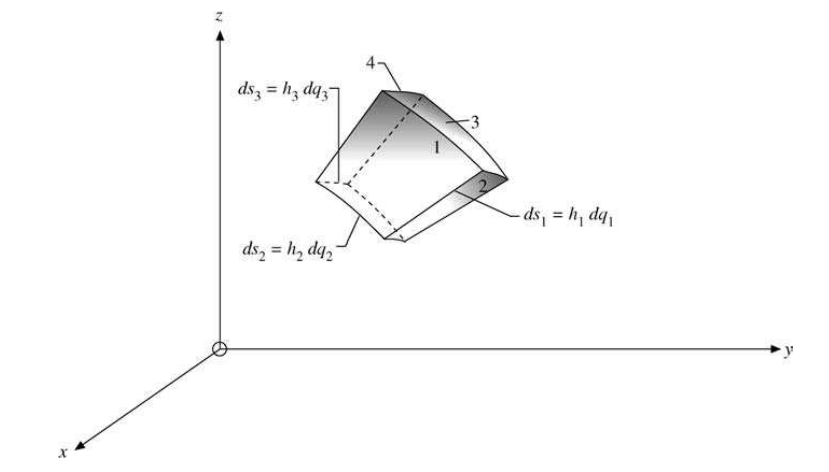
\includegraphics[scale=0.5]{Imagenes/ElementoVolumen_01.png}
    \caption{Elemento de volumen curvilíneo.}
    \label{fig:figura_001}
\end{figure}
Nótese que las direcciones positivas se han elegido tal que $(\vu{q}_{1}, \vu{q}_{2}, \vu{q}_{3})$ o $(\vu{e}_{1}, \vu{e}_{2}, \vu{e}_{3})$ forman un conjunto con orientación derecha: $\vu{q}_{1} \cp \vu{q}_{2} = \vu{q}_{3}$.
\par
La diferencia de área de las integrales para las dos caras de $q_{1} = \text{constante}$ está dada por:
\begin{align}
\begin{aligned}
\left[ V_{1} \: h_{2} \: h_{3} + \pdv{q_{1}} \: (V_{1} \: h_{2} \: h_{3}) \dd{q_{1}} \right] \dd{q_{2}} \dd{q_{3}} -& V_{1} \: h_{2} \: h_{3} \: \dd{q_{2}} \dd{q_{3}} \\
=& \pdv{q_{1}} (V_{1} \: h_{2} \: h_{3}) \dd{q_{1}} \dd{q_{2}} \dd{q_{3}}
\end{aligned}
\label{eq:ecuacion_02_20}
\end{align}
Aquí  $\vb{V}_{i} = \vb{V} \cdot \vu{q}_{i}$ es la proyección de $\vb{V}$ en la dirección de $\vu{q}_{i}$. Sumando los resultados que se obtienen de manera similar para las otras dos superficies, tenemos que:
\begin{align*}
\int \vb{V} (q_{1}, q_{2}, q_{3}) \cdot \dd{\vb{\sigma}} &= \left[ \pdv{q_{1}} (V_{1} \: h_{2} \: h_{3}) + \pdv{q_{2}} (V_{2} \: h_{3} \: h_{1}) + \right. \\
+& \left. \pdv{q_{3}} (V_{3} \: h_{1} \: h_{2}) \right] \dd{q_{1}} \dd{q_{2}} \dd{q_{3}}
\end{align*}
Usando la ecuación (\ref{eq:ecuacion_02_19}), dividiendo por el diferencial de volumen, se tiene que
\begin{align}
\div{\vb{V}} (q_{1}, q_{2}, q_{3}) = \dfrac{1}{h_{1} \: h_{2} \: h_{3}} \; \left[ \pdv{q_{1}} (V_{1} \: h_{2} \: h_{3}) + \pdv{q_{2}} (V_{2}  \:h_{3} \: h_{1}) + \pdv{q_{3}} (V_{3} \: h_{1} \: h_{2})   \right]
\label{eq:ecuacion_02_21}
\end{align}
De las ecuaciones (\ref{eq:ecuacion_02_18}) y (\ref{eq:ecuacion_02_21}), obtenemos el operador Laplaciano, usando $\vb{V} = \grad{\psi} (q_{1}, q_{2}, q_{3})$. Lo que nos devuelve
\begin{align}
\begin{aligned}
\grad \cdot \grad{\psi} (q_{1}, q_{2}, q_{3}) &= \dfrac{1}{h_{1} \: h_{2} \: h_{3}} \left[ \pdv{q_{1}} \left( \dfrac{h_{2} \: h_{3}}{h_{1}} \: \pdv{\psi}{q_{1}} \right) + \right. \\
&+ \left.  \pdv{q_{2}} \left( \dfrac{h_{3} \: h_{1}}{h_{2}} \: \pdv{\psi}{q_{2}} \right) + \pdv{q_{3}} \left( \dfrac{h_{1} \: h_{2}}{h_{3}} \: \pdv{\psi}{q_{3}} \right) \right]  
\end{aligned}
\label{eq:ecuacion_02_22}
\end{align}
\subsection{Rotacional.}
Para desarrollar el rotacional $\curl{\vb{V}}$, usamos el teorema de Stokes, en conjunto con la divergencia, tomamos el límite cuando el elemento de superficie tiende a cero. Trabajando un componente a la vez, consideramos un elemento diferencial de superficie en la superficie curvilínea $q_{1} = \text{constante}$. A partir de:
\begin{align}
\int_{s} \curl{\vb{V}} \cdot \dd{\bm{\sigma}} = \vu{q}_{1} \cdot \left( \curl{\vb{V}} \right) \: h_{2} \: h_{3} \dd{q_{2}} \dd{q_{3}}
\label{eq:ecuacion_02_23}
\end{align}
(del teorema del valor medio del cálculo integral) el teorema de Stokes nos devuelve
\begin{align}
\vu{q}_{1} \cdot \left( \curl{\vb{V}} \right) \: h_{2} \: h_{3} \dd{q_{2}} \dd{q_{3}} = \oint \vb{V} \cdot \dd{\vb{r}}
\label{eq:ecuacion_02_24}
\end{align}
de modo que la integral de línea que rodea la superficie $q_{1}=\text{constante}$. Siguiendo el bucle $(1, 2, 3, 4)$ de la figura (\ref{fig:figura_002})
\begin{figure}[H]
    \centering
    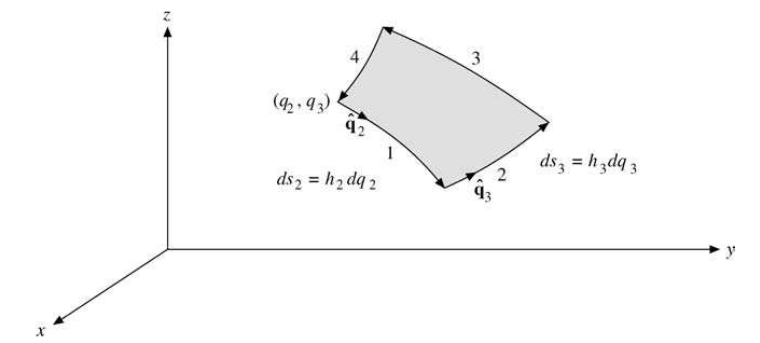
\includegraphics[scale=0.5]{Imagenes/ElementoCurvilineo_02.png}
    \caption{Elemento de superficie curvilíneo con $q_{1}=$ constante.}
    \label{fig:figura_002}
\end{figure}
\begin{align}
\begin{aligned}
\oint \vb{V} (q_{1}, q_{2}, q_{3}) \cdot \dd{\vb{r}} &= V_{2} \: h_{2} \dd{q_{2}} + \left[ V_{3} \: h_{3} + \pdv{q_{2}} (V_{3} \: h_{3}) \dd{q_{2}} \right] \dd{q_{3}} \\
&- \left[ V_{2} \: h_{2} + \pdv{q_{3}} (V_{2} \: h_{2}) \dd{q_{3}} \right] \dd{q_{2}} - V_{3} \: h_{3} \dd{q_{3}} \\
&= \left[ \pdv{q_{2}} (h_{3} \: V_{3}) - \pdv{q_{3}} (h_{2} \: V_{2}) \right] \dd{q_{2}} \dd{q_{3}}
\end{aligned}
\label{eq:ecuacion_02_25}
\end{align}
Se da un signo positivo cuando vamos en la dirección positiva de las partes 1 y 2, y un signo negativo en las partes 3 y 4, ya que vamos en dirección negativa. Los términos de orden mayor en la expansión de la serie de Maclaurin o de Taylor se omiten, ya que tienden a cero cuando el límite del elemento de superficie se hace muy pequeño ($\dd{q_{2}} \rightarrow 0, \dd{q_{3}} \rightarrow 0$.)
De la ecuación (\ref{eq:ecuacion_02_24}) tenemos
\begin{align}
\curl{\vb{V}} \eval_{1} = \dfrac{1}{h_{2} \: h_{3}} \; \left[ \pdv{q_{2}} (h_{3} \: V_{3}) - \pdv{q_{3}} (h_{2} \:V_{2}) \right]
\label{eq:ecuacion_02_26}
\end{align}
Las dos componentes que restan de $\curl{\vb{V}}$, se obtienen al realizar una permutación ciclíca de los índices. La mejor manera para escribir el rotacional, es una forma de determinante
\begin{align}
\curl{\vb{V}} = \dfrac{1}{h_{1} \: h_{2} \:h_{3}} \mdet{
\vb{q}_{1} \: h_{1} & \vb{q}_{2} \: h_{2} & \vb{q}_{3} \: h_{3} \\[1em]
\displaystyle \pdv{q_{1}} & \displaystyle \pdv{q_{2}} & \displaystyle \pdv{q_{3}} \\[1em]
h_{1} \: V_{1} & h_{2} \: V_{2} & h_{3} \: V_{3}
}
\label{eq:ecuacion_02_27}
\end{align}
Recordemos que debido a la presencia de los operadores diferenciales, este determinante debe de expandrise de arriba hacia abajo. La ecuación en sí, no es idéntica a la forma del producto cruz de dos vectores, ya que $\grad$ no es un vector común, es un operador vectorial.
\end{document}
